% !TEX root = ../foresight.tex

\section{Planning For Exploration}

Planning a path to observe the blind spots of an autonomous car is broken into
following steps. First, using the 2D laser scan from the car, we compute a
bounding polygon. This polygon represents the known free space where the
quadrotor can travel. We use the laser scan to determine regions in space where
that the car is not able to sense. These regions are called blind regions. A
path is then computed for the quadrotor that maximizes the observed area of the
blind regions while staying within the bounding polygon for a given time
horizon.

The remainder of this section is structured as follows; Sec.~\ref{sec:poly}
introduces the our formal definition of a laser scan and describes how the
bounding polygon is found, Sec.~\ref{sec:blindregions} describes how the blind
regions are computed from the laser scan, and Sec.~\ref{sec:planner} describes
and analyzes the algorithm we developed for computing the exploratory path.

\begin{figure}[ht]

    \centering

    \begin{subfigure}[t]{0.44\textwidth}
        \centering
        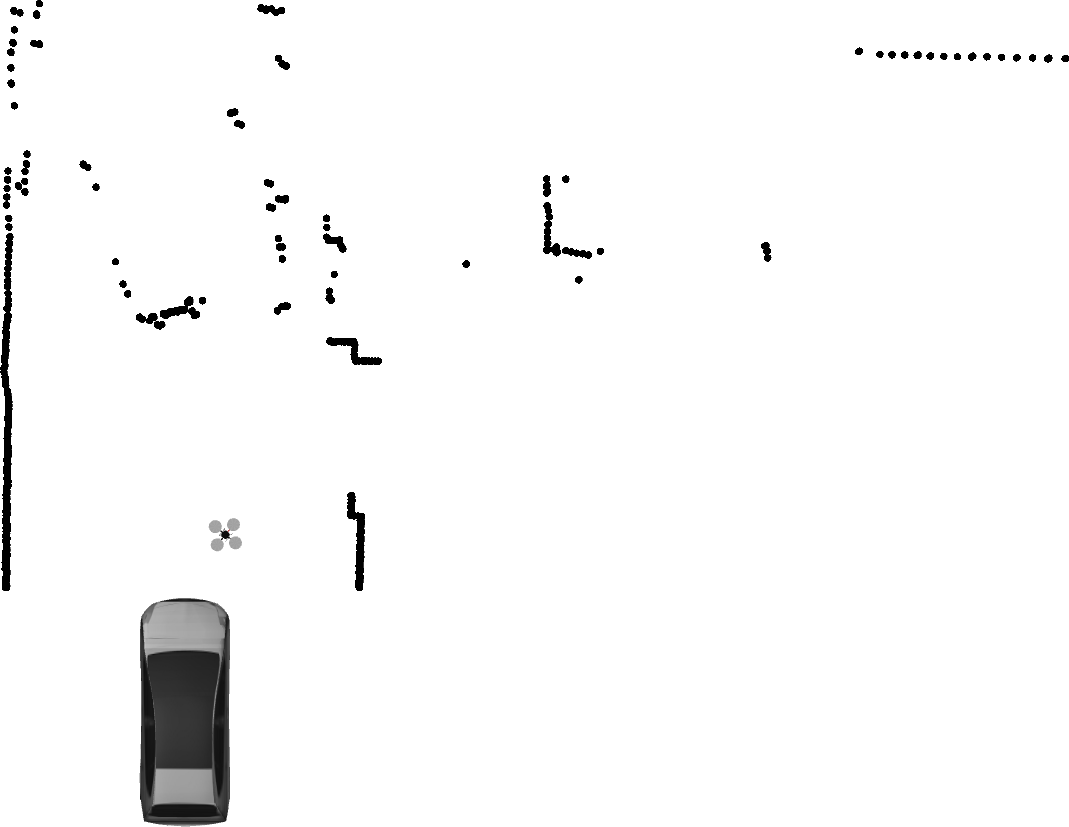
\includegraphics[width=1\linewidth]{01laser}
        \caption{}
        \label{fig:01laser}
    \end{subfigure}
    ~
    \begin{subfigure}[t]{0.44\textwidth}
        \centering
        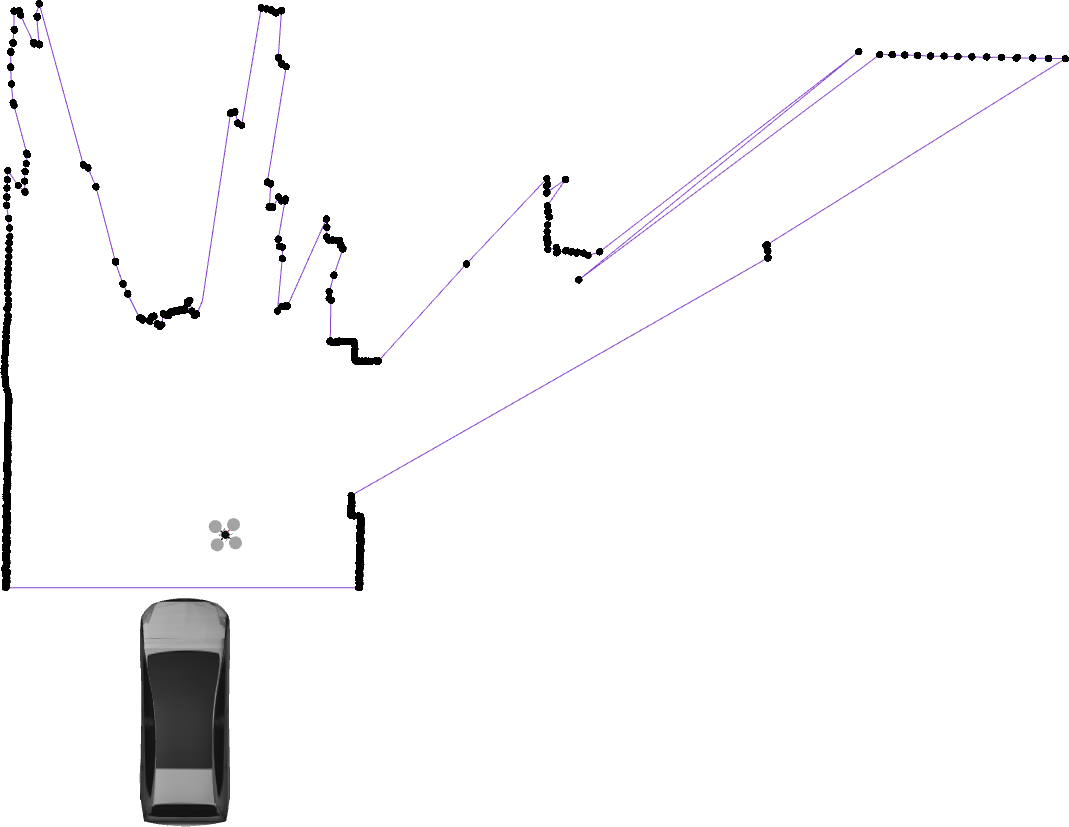
\includegraphics[width=1\linewidth]{02polygon}
        \caption{}
        \label{fig:02polygon}
    \end{subfigure}
    ~
    \begin{subfigure}[t]{0.44\textwidth}
        \centering
        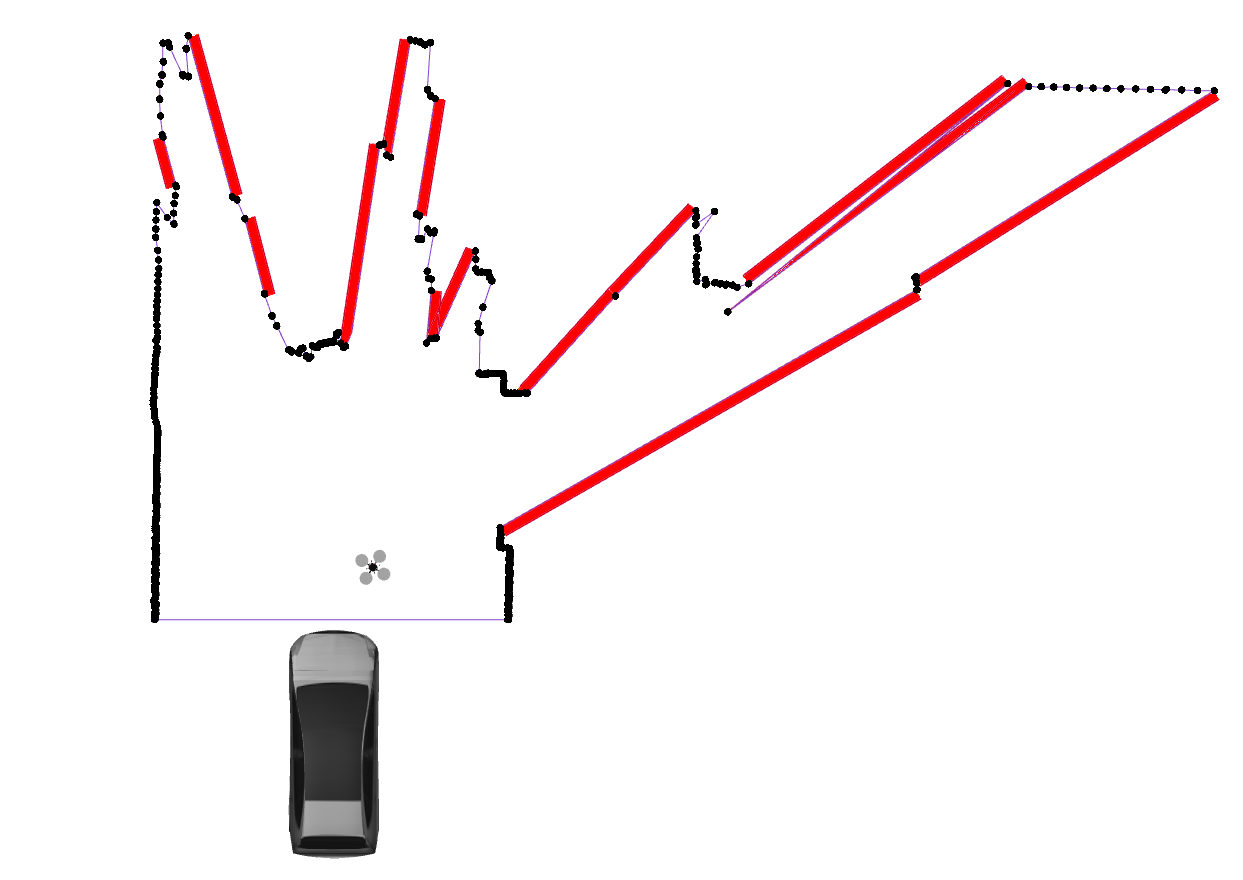
\includegraphics[width=1\linewidth]{03blindregions}
        \caption{}
        \label{fig:03blindregions}
    \end{subfigure}
    ~
    \begin{subfigure}[t]{0.44\textwidth}
        \centering
        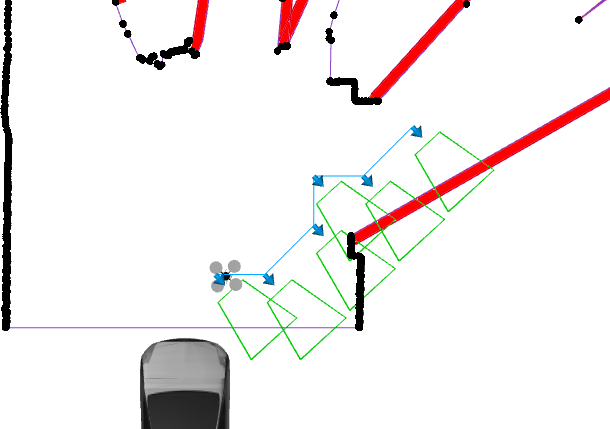
\includegraphics[width=1\linewidth]{04planner-small}
        \caption{}
        \label{fig:04planner-small}
    \end{subfigure}

    \caption{Plots showing the four stages of the planner. Fig. (a) shows the
    points from the laser scan. Fig. (b) shows bounding polygon created from
the laser scan. Fig. (c) shows the regions occluded to the vehicle in red and
Fig. (d) shows the initial plan for the quadrotor to view some of these blind
regions.}

    \label{fig:planner-stages}

\end{figure}

\subsection{Finding the Bounding Polygon}

\label{sec:poly}

The bounding polygon computed using a scan from the 2D LiDAR sensor on the car
is used as a conservative representation of the free space in which the
quadrotor can travel. Below we provide a formal definition of a laser scan that
is used in the rest of the paper.

\begin{definition}

    A laser scan is a sequence of points, $L = \{\mathbf{c} + r_i \cdot [\cos
    \theta_i, \sin \theta_i] ^ T : \theta_{\min} \leq \theta_i \leq
    \theta_{\max} \} \subset \R^2$, where $\mathbf{c}$ is the 2D position of
    the LiDAR sensor, $r_i$ is the distance from the sensor to the closest
    obstruction in the $\theta_i$ direction, and
    $[\theta_{\min}$, $\theta_{\max}]$ is the angular range of the sensor.

\end{definition}

From the laser scan, we compute a bounding polygon. The bounding
polygon is defined as the minimum area simple polygon that contains all the
points in the laser scan. Since the laser scan data is ordered by $\theta_i$
from $\theta_{\min}$ to $\theta_{\max}$, the bounding polygon can be
constructed in one pass with the vertex sequence $\{\mathbf{c}\} \cup L \cup
\{\mathbf{c}\}$. Fig.~\ref{fig:02polygon} shows an example of laser scan
data and the corresponding bounding polygon.

\subsection{Determining the Blind Regions}

\label{sec:blindregions}

Using the laser scan data, we can determine which areas in the environment the
car is unable to sense. We call these areas blind regions. The blind region,
$\B$, is the set of points contained within a rectangle with a vertex sequence
$\{L_i, L_i + k \cdot \hat{L}_{i, i + 1}, L_{i + 1} + k \cdot \hat{L}_{i, i +
1}, L_{i + 1}, L_i\}$ where $\hat{L}_{i, i + 1}$ is the unit normal for the
vector between points $L_i$ and $L_{i + 1}$ that points away from the bounding
polygon and $k$ is a tuning parameter that contributes to the area of the blind
region. In practice we only care for blind regions where $||L_i - L_{i + 1}||_2
> \delta$ where $\delta$ is a tuning parameter because the laser scan consists
of a finite number of points with a known angular distance. We will use $\B$ to
denote the set of all such regions.  Fig.~\ref{fig:03blindregions} shows an
example of blind regions in found in a found from a laser scan.

% maybe can change the name of this section
\subsection{Computing the Exploratory Path}

\label{sec:planner}

Using the blind regions, current configuration of the quadrotor, and the
bounding polygon, we present an anytime algorithm that computes a collision
free path for the quadrotor that maximizes the total observed area of the blind
regions within a given time horizon. The algorithm builds a search tree
starting from the current configuration of the quadrotor. It expands leaf nodes
in descending order of total observed blind region area and only adds new leaf
nodes to the search that are contained within the bounding polygon. When a
collision free neighbour is propagated, the orientation, $\theta^*(x, \B)$,
that maximizes the area of the remaining blind region, $\B$, viewed at that
configuration, $x$, is also added to the search tree. Below we formally define
this orientation.

\begin{definition}

    Let $\psi(x, \theta, \B)$ be the set of points visible by the quadrotor at
    position $x \in \R^3$ with orientation $\theta$. Let $\theta^*(x, \B) =
    \argmax{0 < \theta \leq 2\pi} \psi(x, \theta, \B)$. For convenience, we
    define $\psi^*(x, \B) = \psi(x, \theta^*(x, \B), \B)$.
    % \ja{What are the visiblie points?}

\end{definition}

As the quadrotor follows the path, the planner is constantly replanning. To
avoid oscillating between candidate paths, the quadrotor only follows a new
path if its current path is no longer collision free or if the new path has a
larger objective value. % \ja{ADD caption to algorithm and figure!}

\begin{algorithm}[h!]
    \caption{Path planning for remote sensing UAV (looking around the corner)}
    \algorithmicrequire{\begin{itemize}
            \item $x_0$: The initial position of the robot,
                $\B$: The blind region, $\Poly$: The bounding polygon
        \end{itemize}}
    \algorithmicensure{\begin{itemize}
            \item $\Pi \subset \R^3 \times [0, 2\pi]$: A sequence of 3D positions
                and orientations representing the path
        \end{itemize}}
    \label{algo:find_path}
    \begin{algorithmic}[1]
        \setcounter{ALC@line}{0}
        % \vspace*{1mm}

        \STATE $Q \leftarrow \{(x_0, \theta^*(x_0, \B),
            \B \, \backslash \, \psi^*(x_0, \B))\}$
        \WHILE{$|Q| > 0$}

        \STATE $(x, \theta, \rB) \leftarrow \argmin{\rB \in Q} \Area(\rB)$

            \IF{$\Function{SearchTimeoutExpired}()$}
                \STATE $\Pi \leftarrow \{\}$
                \WHILE{$\Function{HasParent}(x, \theta)$}
                    \STATE $\Pi \leftarrow \Pi \cup \{x\}$
                    \STATE $(x, \theta) \leftarrow \Function{Parent}(x, \theta)$
                \ENDWHILE
                \RETURN $\Pi$
            \ENDIF
            \FORALL{$x' \in \Function{CollisionFreeNeighbours}(x, \Poly)$}
            \STATE $\theta' \leftarrow \theta^*(x', \rB)$
            \STATE $Q \leftarrow Q \cup \{(x', \theta', \rB \, \backslash \,
                    \psi^*(x', \rB))\}$
                \STATE $\Function{Parent}(x', \theta') \leftarrow (x, \theta)$
            \ENDFOR
            \STATE $Q \leftarrow Q \, \backslash \, \{(x, \theta', \rB)\}$
        \ENDWHILE
        \RETURN $\{\}$

    \end{algorithmic}
\end{algorithm}

At the start of Algo.~\ref{algo:find_path}, we initialize a priority queue that
is used to store the leaf nodes of the search tree. Each node is comprised of
the position of the quadrotor, $x \in \R^3$, the orientation of the quadrotor
on the Z-axis, $\theta \in [0, 2\pi]$, and the remaining blind region, $\B$,
that is left unobserved after the quadrotor reaches $x$ with orientation
$\theta$. Until the search timeout has expired, collision free neighbours of
$x$ are added to the search along with their maximizing orientation and
remaining unobserved blind regions.  Once the search has expired, the path,
$\Pi$ comprised of 3D positions and orientations, that was able to view the
largest cumulative blind region area starting from $x_0$ is returned.
Fig.~\ref{fig:04planner-small} shows an example of a path being computed to
view the blind regions.

\subsection{Autonomous Landing}

To enable autonomous landing, the quadrotor tries to maintain a static position
relative to the car as it drives towards a parking spot. Once the vehicle has
stopped, the quadrotor moves directly above the landing platform and proceeds
to land on the platform.
